\documentclass[12pt,a4paper]{article}
\usepackage[utf8]{inputenc}
\usepackage[T1]{fontenc}
\usepackage{textcomp}
\usepackage{amsmath}
\usepackage{amsfonts}
\usepackage[francais]{babel}
\usepackage{amssymb}
\usepackage{graphicx}
\usepackage[top=2.00cm]{geometry}
\usepackage{enumitem}
%\usepackage{mathtools}
\usepackage{bigcenter}
\usepackage{multicol}
%\usepackage{minibox}

%Modif des enumerates numeros en gras. leftmargin=*,
\setlist[enumerate]{label=\textbf{\arabic*}.}

\usepackage{titlesec}
\renewcommand{\thesection}{\Roman{section}}
%modif des titres de section diminuer la taille
\titleformat{\section}
  {\normalfont\Large\bfseries\scshape}{\thesection}{1em}{}
\titleformat{\subsection}
  {\normalfont\large\bfseries}{\thesubsection}{1em}{}


\author{CHARNAY Valentin, FINOT Sylvain}
\title{Compte rendu de TP :\\ \scshape Ondes Centimétriques}

\begin{document}
\maketitle
\rule{\linewidth}{0.4pt}
\section{\scshape Antenne cornet}
\subsection{Nature et polarisation de l'onde}
Dans cette partie, on souhaite déterminer la nature de l'onde émise par l'antenne cornet (constituée d'une diode Gunn). Pour ce faire, nous plaçons une antenne réceptrice a une distance "d" variable et nous mesurons la tension "A" (continue) à ses bornes à l'aide d'un oscilloscope.\\
On trace par la suite
$$\ln A = f(\ln D)$$
\begin{bigcenter}
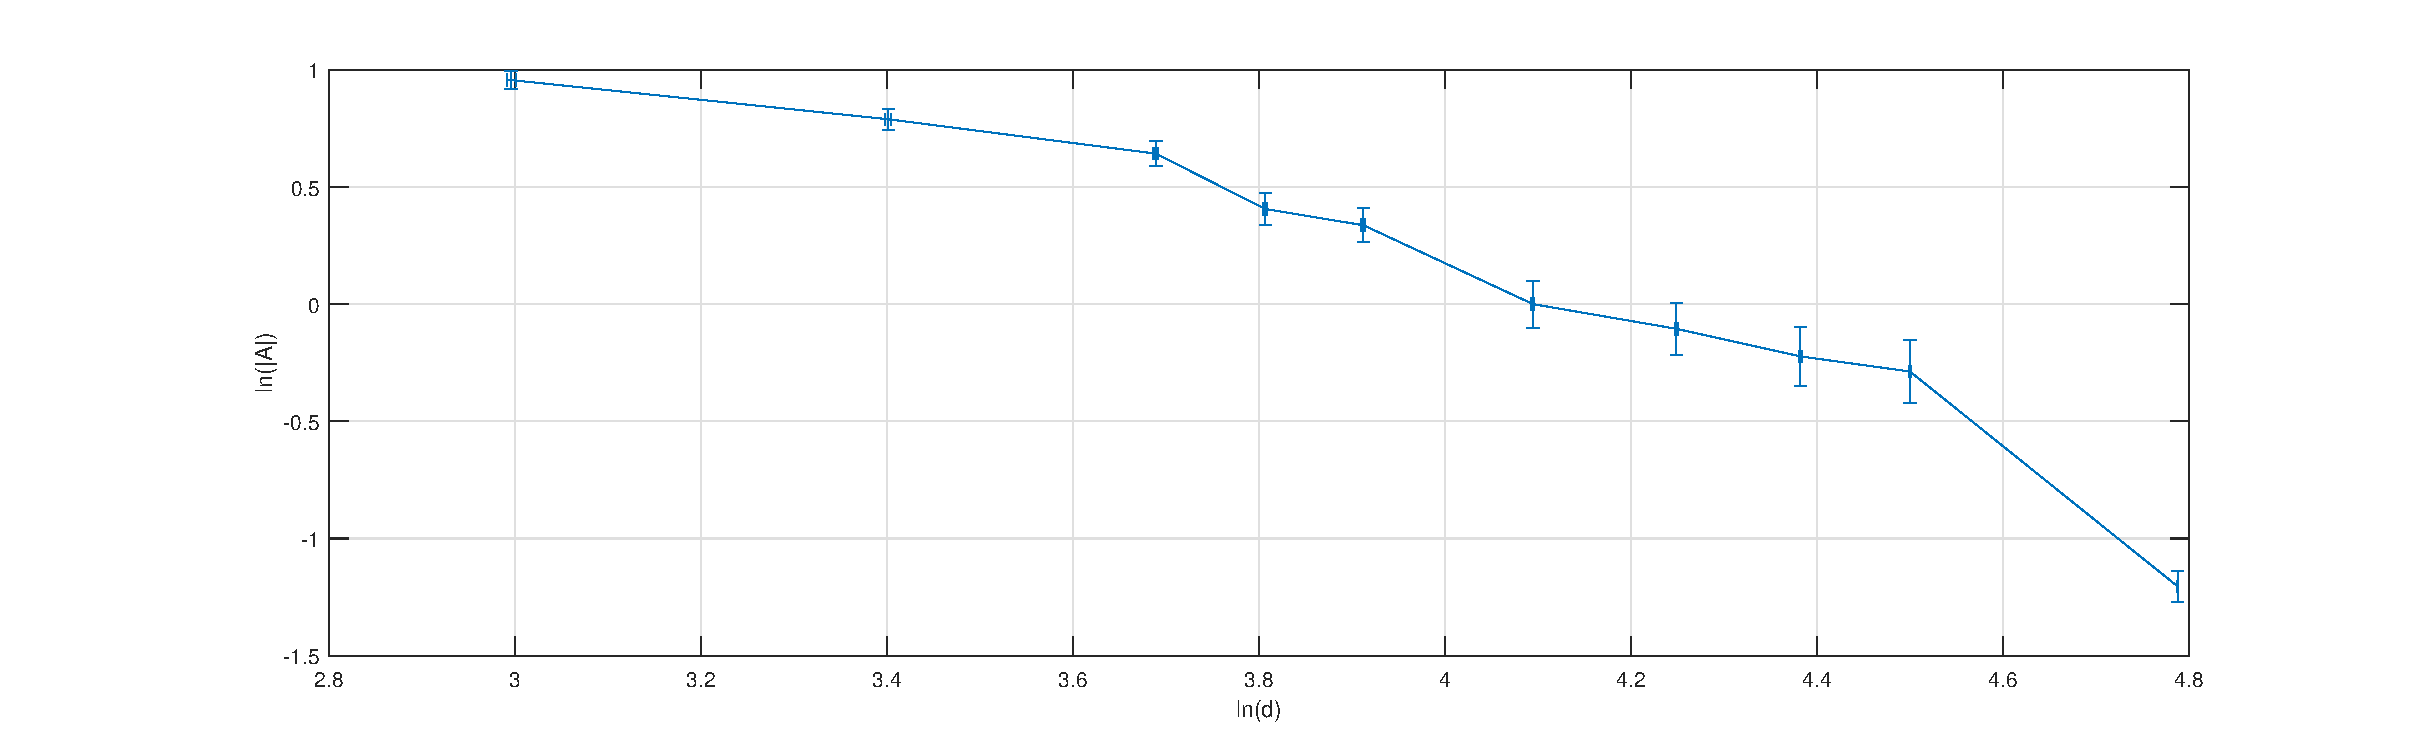
\includegraphics[scale=0.5]{matlab/lnA}
\end{bigcenter}
On remarque que la tension aux bornes de l'antenne diminue en l'éloignant de l'émetteur, on peut donc en conclure que les ondes émises ne sont pas des ondes planes. On en déduit donc qu'il s'agit d'une onde sphérique mais concentrée par le cornet. Les barres d'erreur du graphe ci-dessus sont calculées à partir d'incertitudes de lectures. On estime que les incertitudes sont de l'ordre de la plus petite graduation, on néglige les éventuelles fluctuations de la tension A. Ainsi $\Delta d$ vaut 1mm et $\Delta A$ vaut (1/5) du calibre de l'oscilloscope.
Afin de déterminer une éventuelle polarisation de l'onde, il suffit de faire pivoter l'antenne par rapport à l'axe "Emetteur-Récepteur". On remarque alors qu'après rotation de 90° (i.e l'antenne parallèle au sol), la tension est nulle, ce qui implique que l'onde est polarisée.
\subsection{Diagramme de rayonnement}
On s'intéresse maintenant au diagramme de rayonnement de l'antenne.
%DIAGRAMME RAYONNEMENT

\section{Ondes centimétriques libres}
\subsection{Ondes stationnaires}
En plaçant une plaque métallique face au cornet à une distance d'environ 20cm, celui ci agit comme un miroir. Il s'établit alors un régime d'ondes stationnaires entre le cornet et la plaque métallique (superposition de l'onde incidente et de l'onde réfléchie). En déplaçant l'antenne réceptrice entre le cornet et la plaque, on observe une série de maxima et de minima. La distance entre deux maximums successifs est $\lambda$/2 où $\lambda$ est la longueur d'onde des ondes centimétriques. On relève quelques points:
\begin{center}
\begin{tabular}{|c|c|}
	\hline 
	Maximum n° & d (cm) \\ 
	\hline 
	1 & 15 \\ 
	\hline 
	2 & 13.25 \\ 
	\hline 
	3 & 11.75 \\ 
	\hline 
	4 & 10 \\ 
	\hline 
	5 & 6.7 \\ 
	\hline 
\end{tabular} 
\end{center}
Pour plus de précision, on calcule en prenant 5 maxima : 
\setlength\columnseprule{0.5pt}
\begin{multicols}{2}
\begin{align*}
15-6,7 &= \dfrac{5\lambda}{2}\\
\implies \lambda &= \dfrac{2(15-6,7)}{5}=3,32 \text{ cm}
\end{align*}
\vfill
\columnbreak
\begin{align*}
\Delta \lambda &= \sqrt {\left( \Delta d_{1}\right) ^{2}+\left( \Delta d_{2}\right) ^{2}}\\
\implies \Delta \lambda &= \sqrt {0,1^2+0,1^2}=0,14 \text{ cm}
\end{align*}
\end{multicols}
$\lambda = 3,32\pm1,4.10^{-1}$ cm\\
Comparons ce résultat aux données constructeur : Fréquence d'émission 9,35GHz.
\begin{align*}
c &= \lambda.\nu\\
\iff \lambda &= \dfrac{c}{\nu}\\
&=\dfrac{c}{9,35.10^9}\\
&=3,2 \text{ cm}
\end{align*}
Le résultat expérimentale correspond bien aux données fournies par le constructeur. 
\end{document}